\documentclass[conference]{IEEEtran}
\IEEEoverridecommandlockouts
\usepackage{cite}
\usepackage{amsmath,amssymb,amsfonts}
\usepackage{graphicx}
\usepackage{booktabs}
\usepackage{xcolor}
\usepackage{algorithm}
\usepackage{algpseudocode}
\usepackage{tikz}
\usetikzlibrary{arrows.meta,positioning,fit,backgrounds}
\usepackage[hidelinks]{hyperref}
\graphicspath{{../results/figures/}}
\newcommand{\eps}{\varepsilon}
\usepackage{placeins}
\renewcommand{\topfraction}{0.92}\renewcommand{\bottomfraction}{0.8}\renewcommand{\textfraction}{0.06}
\renewcommand{\floatpagefraction}{0.85}\renewcommand{\dbltopfraction}{0.92}\renewcommand{\dblfloatpagefraction}{0.85}
\setcounter{topnumber}{3}\setcounter{bottomnumber}{2}\setcounter{totalnumber}{5}\setcounter{dbltopnumber}{2}

\begin{document}

\title{StreamHybridSketch: Federated Linear Sketches with Continual-Release Differential Privacy for Streaming Heavy Hitters}

% TODO(team): replace placeholders with the four team members and affiliation
\author{\IEEEauthorblockN{Member One, Member Two, Member Three, Member Four}
\IEEEauthorblockA{\textit{IOE413 Streaming Data Analytics -- Team 22}\\
\textit{Department / University (placeholder)}}}

\maketitle

\begin{abstract}
Live statistics such as trending words or popular places are often computed from data that
lives on user devices or in separate organisations. Federated linear sketches combined with
secure aggregation and differential privacy (DP) let a server estimate frequencies without seeing raw
events, but existing methods target a fixed dataset analysed in a few rounds. We build an
end-to-end streaming pipeline---Kafka ingestion, eight Flower edge clients with X25519 pairwise-mask
secure aggregation and distributed Gaussian noise, a Flower server strategy, a release topic, an
evaluator and a Grafana dashboard---and reproduce three base methods inside it: DP-HybridSketch
(Wu et al., NeurIPS'23), TrieHH (Zhu et al., AISTATS'20) and IBLT-based heavy-hitter recovery
(Gasc\'on et al., FL@ICML'23). On top of the per-window DP-HybridSketch baseline we add
binary-tree continual release, a heavy-hitter \emph{peeling} estimator for shared-sign tree nodes,
adaptive two-phase sketch width, a top-$k$ drift detector and an invertible (IBLT) layer.
On Gowalla, Sentiment140 and a synthetic drifting Zipf stream, the drift-aware per-round variant recovers
heavy-hitter F1 after an abrupt drift in 1.5 instead of 5.5 rounds and cuts upload by 31--61\% on two datasets at
equal privacy; tree release with peeling halves the cumulative $\ell_\infty$ error at a small budget ($\eps=0.125$).
We also report where the enhancements do \emph{not} help: tree release loses on sliding windows and at
$\eps\ge 1$, and the IBLT layer costs 2--4$\times$ more communication than a dictionary-assisted CountSketch.
\end{abstract}

\begin{IEEEkeywords}
federated analytics, count sketch, differential privacy, continual release, secure aggregation, heavy hitters, Kafka, Flower
\end{IEEEkeywords}

\section{Introduction}
Keyboards that learn new words, maps that surface busy places and hospitals that share error codes all need
\emph{live} frequency statistics over data they should not centralise. Federated analytics keeps the data local
and moves only compact summaries; \emph{linear} sketches such as CountSketch~\cite{charikar2002} are a natural choice because the
server can add them under secure aggregation (SecAgg) and learn only the sum~\cite{wu2023,bonawitz2017}.
Real data, however, is an unbounded stream whose distribution drifts, and a system that keeps releasing
statistics must account for the privacy it spends across all releases. Existing federated sketch methods analyse a
fixed population in one or a handful of rounds~\cite{wu2023,zhu2020,gascon2023}.

\textbf{Problem.} Estimate item frequencies and top-$k$ heavy hitters over distributed, drifting event streams with
federated linear sketches, SecAgg and DP, keeping error, per-client communication and cumulative privacy loss low.
A batch system cannot answer this (it needs a release every window), and a single tool cannot either: we need a
log (Kafka), federated orchestration (Flower), cryptographic aggregation, a DP accountant and a live dashboard.

\textbf{Contributions.}
(1)~A working streaming pipeline with real data flowing Kafka $\rightarrow$ Flower edges $\rightarrow$ SecAgg
$\rightarrow$ server $\rightarrow$ Kafka $\rightarrow$ InfluxDB/Grafana, and an offline harness that runs the
\emph{identical} protocol code (bit-identical aggregates, verified). (2)~Reproductions of the core claims of
three base papers on public data. (3)~StreamHybridSketch: tree continual release, a peeling estimator, adaptive
width, drift detection and an IBLT layer, each ablated. (4)~An honest quantitative comparison, including negative
results and the regime boundaries of each component.

\section{Related Work and Gap}
\textbf{Wu et al.~\cite{wu2023} (primary baseline).} \emph{Question:} how should a CountSketch under SecSum be sized
and reused across rounds, with and without DP? \emph{Data:} Gowalla (grid, $d{=}175$k), C4, Sentiment140.
\emph{Metrics:} $\ell_\infty$ error, sketch size/communication, $(\eps,\delta)$. \emph{Findings:} the necessary width depends on
the tail of the frequency vector, so a two-phase method (fit a power law to a small probe sketch, then size the sketch)
matches the instance-optimal width; in multi-round settings HybridSketch---shared bucket hash, fresh sign hash each
round---beats SharedSketch and FreshSketch; DP-HybridSketch (Gaussian noise per released sketch) is near minimax-optimal.
\emph{Model:} no learned model.

\textbf{Zhu et al.~\cite{zhu2020} (TrieHH).} \emph{Question:} can heavy hitters be discovered from on-device data with central DP
and minimal disclosure? \emph{Data:} Sentiment140 (1.6M tweets, 650k users). \emph{Metrics:} precision/recall/F1 of top
words vs.\ $\eps$. \emph{Findings:} sampling $\gamma\sqrt n$ users per round and keeping trie prefixes with $\ge\theta$ votes is
$(\eps,\delta)$-DP without added noise, and recovers most top words at single-digit $\eps$. \emph{Model:} none (interactive trie).

\textbf{Gasc\'on et al.~\cite{gascon2023}.} \emph{Question:} what are the communication limits of multi-round heavy-hitter
recovery when clients may only send linear sketches? \emph{Data:} Stack Overflow (TFF), 3-character prefixes.
\emph{Metrics:} F1 vs.\ per-user communication and rounds. \emph{Findings:} frequency oracles (CountSketch, Count-Min)
are suboptimal; IBLTs~\cite{goodrich2011} with local threshold sampling reach F1$=0.8$ with $\sim$10$\times$ less communication.
\emph{Model:} none.

\textbf{Gap.} All three release statistics a fixed number of times over a static population. A stream needs a
release \emph{every} window, so (i) noise accumulates or privacy loss composes over time, (ii) the right sketch width
changes as the distribution changes, and (iii) sliding-window statistics must react to drift. The binary-tree
mechanism~\cite{dwork2010,chan2011} answers (i) for scalar counters but, as we show, interacts badly with
HybridSketch's fresh signs; no prior work combines it with federated sketches.

\section{System Architecture}
Fig.~\ref{fig:arch} shows the pipeline. A \textbf{producer} replays a dataset in event-time order into Kafka topic
\texttt{events}, one partition per edge (users are hashed to 8 edges), and appends a watermark to every partition
when a window closes. Each \textbf{edge} is a Flower client that consumes only its partition. In Flower round $1$
it publishes an X25519 public key; in round $2{+}t$ it waits for watermark $t$, samples one item per local user,
builds the payload of every configured variant (sketch nodes, its share of the Gaussian noise, optional IBLT),
masks it with pairwise HKDF-derived PRG masks and returns it. The \textbf{Flower server} (custom
\texttt{Strategy}) plans each round (node set, widths, hash seeds, noise scale, IBLT threshold), sums the masked
payloads modulo $2^{64}$ (masks cancel), decodes each variant, updates drift and width state, and publishes a
release (top-$k$ for the sliding window and the cumulative stream) to Kafka topic \texttt{releases}. An
\textbf{evaluator} (not part of the protocol) recomputes exact ground truth from \texttt{events}, scores every
release and writes metrics to \textbf{InfluxDB}, visualised live in \textbf{Grafana}.

\begin{figure*}[t]
\centering
\resizebox{\textwidth}{!}{%
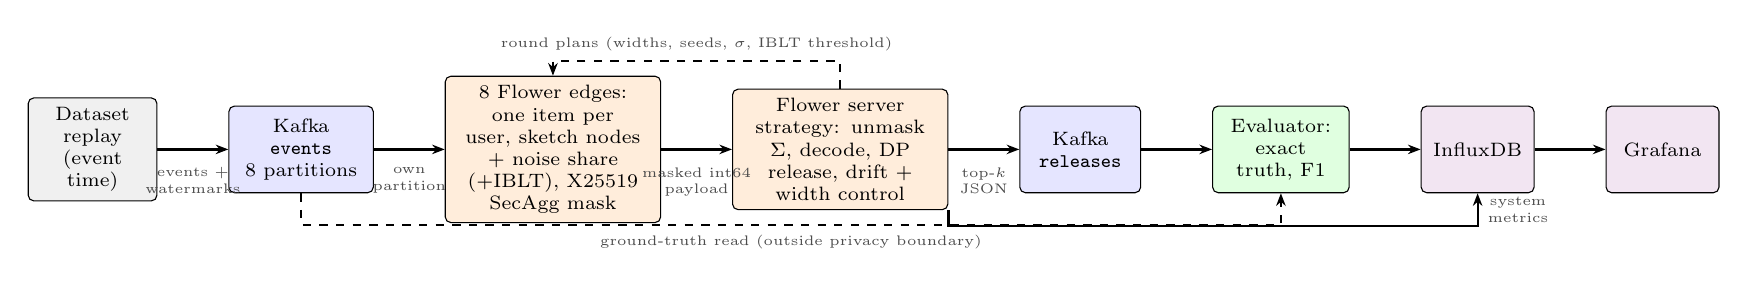
\begin{tikzpicture}[font=\scriptsize, node distance=4mm and 9mm,
  box/.style={draw, rounded corners=2pt, align=center, minimum height=11mm, text width=#1},
  box/.default=17mm, ar/.style={-{Stealth[length=1.6mm]}, thick}, lbl/.style={font=\tiny, align=center, text=black!70}]
\node[box=14mm, fill=gray!12] (data) {Dataset replay\\(event time)};
\node[box=16mm, fill=blue!10, right=of data] (kafka) {Kafka\\\texttt{events}\\8 partitions};
\node[box=25mm, fill=orange!14, right=of kafka] (edges) {8 Flower edges: one item per user, sketch nodes + noise share (+IBLT), X25519 SecAgg mask};
\node[box=25mm, fill=orange!14, right=of edges] (srv) {Flower server strategy: unmask $\Sigma$, decode, DP release, drift + width control};
\node[box=13mm, fill=blue!10, right=of srv] (rel) {Kafka\\\texttt{releases}};
\node[box=15mm, fill=green!12, right=of rel] (ev) {Evaluator: exact truth, F1};
\node[box=12mm, fill=violet!10, right=of ev] (influx) {InfluxDB};
\node[box=12mm, fill=violet!10, right=of influx] (graf) {Grafana};
\draw[ar] (data) -- node[lbl, below=1mm]{events +\\watermarks} (kafka);
\draw[ar] (kafka) -- node[lbl, below=1mm]{own\\partition} (edges);
\draw[ar] (edges) -- node[lbl, below=1mm]{masked int64\\payload} (srv);
\draw[ar] (srv) -- node[lbl, below=1mm]{top-$k$\\JSON} (rel);
\draw[ar] (rel) -- (ev);
\draw[ar] (ev) -- (influx);
\draw[ar] (influx) -- (graf);
\draw[ar, dashed] (srv.north) -- ++(0,3.5mm) -| node[lbl, pos=0.25, above]{round plans (widths, seeds, $\sigma$, IBLT threshold)} (edges.north);
\draw[ar, dashed] (kafka.south) -- ++(0,-4mm) -| node[lbl, pos=0.25, below]{ground-truth read (outside privacy boundary)} (ev.south);
\draw[ar] (srv.south east) -- ++(0,-2mm) -| node[lbl, pos=0.75, right]{system\\metrics} (influx.south);
\end{tikzpicture}}
\caption{Pipeline architecture. Raw events never leave the edge; the server sees only the SecAgg sum of noisy sketches.
Dashed: the control plane (round plans) and the evaluator's ground-truth read.}
\label{fig:arch}
\end{figure*}

\section{Proposed Enhancement: StreamHybridSketch}
\textbf{Privacy model.} Each user contributes one item per window, sampled uniformly from its events (as in
\cite{wu2023,zhu2020}). The privacy unit is one user's contribution to one window---event-level DP under continual
observation~\cite{dwork2010}. A depth-$d$ CountSketch then has $L_2$ sensitivity exactly $\sqrt d$. Each of the $K$ edges
adds $\mathcal N(0,\sigma^2/K)$ (fixed point, $2^{-8}$) so the aggregate carries $\mathcal N(0,\sigma^2)$ and the server never
sees un-noised data. Budgets are calibrated and reported with Google's R\'enyi-DP~\cite{mironov2017} accountant, including a noisy user count released each round.

\textbf{(a) Tree continual release.} The baseline releases each window's sketch once with noise $\sigma_B$; a cumulative
query over $t$ windows then has noise variance $t\sigma_B^2$. We instead release every completed dyadic node of a binary tree
over windows (height $h{=}\lceil\log_2 T\rceil$), so each unit appears in $h{+}1$ releases and any prefix or window is a sum of
$O(\log t)$ nodes. Edges keep their local per-window histograms and re-encode node sketches, so a level-$\ell$
node costs one extra sketch upload every $2^\ell$ rounds (about $2\times$ the baseline upload in total).

\textbf{(b) Peeling estimator.} Tree nodes must be summable, so all nodes share sign hashes---this turns HybridSketch
into a SharedSketch, whose error is driven by heavy items colliding coherently across rounds (Sec.~\ref{sec:res}).
For each node we estimate the top-$P$ ($P{=}200$) candidates, subtract their encoded estimates, read every item from
the residual and add back its own estimate. This is pure post-processing (no privacy cost).

\textbf{(c) Adaptive two-phase width.} Following \cite{wu2023}, the server fits $f_i\approx\beta i^{-\alpha}$ to the top-20 estimates
of the previous release and sets $W=2(\#\{f_i\ge\tau\}+\tau^{-2}\sum_{f_i<\tau}f_i^2)$ (rounded to a power of two, smoothed
over three rounds) for target $\tau$. Widths are powers of two, so sketches of different widths fold exactly.
Because phase 1 reuses the last release, it costs no extra round or privacy.

\textbf{(d) Drift detection.} Each round the server compares the top-50 of the newest window with the top-50 of the
current sliding window. If the Jaccard overlap falls below half its recent mean, it restarts the sliding window at
the current round and resets the width to its maximum.

\textbf{(e) IBLT layer.} Optionally, users threshold-sample their item (keep with probability $1/t$, report value $t$) and
insert it into a 3-hash additive IBLT. The server peels the aggregate to list identities without a candidate
dictionary, and adapts $t$ by feedback on the table's load. This layer is protected by SecAgg and sampling, not DP.

Algorithm~\ref{alg:round} summarises one round of the protocol; the per-round baseline is the special case with only
the leaf node, fixed $W$ and fresh signs.
\begin{algorithm}[t]
\caption{One StreamHybridSketch round (window $t$)}\label{alg:round}
\begin{algorithmic}[1]
\Statex \textbf{Server:} plan $\mathcal P_t$: nodes $\mathcal N_t$ completed at $t$ (tree) or $\{(0,t)\}$; width $W_t$; seeds; $\sigma$; IBLT threshold
\For{each edge $e$ \textbf{in parallel}}
  \State consume partition $e$ until watermark $t$; sample one item per user
  \For{each node $(\ell,j)\in\mathcal N_t$}
     \State $S_e^{(\ell,j)}\gets$ CountSketch of local items in rounds $[j2^\ell,(j{+}1)2^\ell)$, width $W^{(\ell,j)}$
     \State $S_e^{(\ell,j)}\gets S_e^{(\ell,j)} + \mathcal N(0,\sigma^2/K)$ \Comment{noise share}
  \EndFor
  \State optional: threshold-sample items, encode IBLT $B_e$
  \State send $\mathrm{mask}_e([S_e,B_e])$ \Comment{$\sum_e \mathrm{mask}_e(x_e)=\sum_e x_e \bmod 2^{64}$}
\EndFor
\State \textbf{Server:} $S\gets\sum_e$ payloads; store nodes; peel IBLT
\State estimate window / cumulative frequencies from the dyadic cover (with peeling); release top-$k$ to Kafka
\State drift test (top-$k$ Jaccard) $\Rightarrow$ reset window; two-phase fit $\Rightarrow W_{t+1}$; IBLT load $\Rightarrow$ threshold
\end{algorithmic}
\end{algorithm}

From the ablations we recommend two configurations: \textbf{SHS-W} (per-round release + (c) + (d)) for
sliding-window and current-trend queries, and \textbf{SHS-C} (tree (a) + peeling (b) + (d), fixed width) for long-horizon
cumulative statistics at small $\eps$.

\begin{figure*}[t]\centering
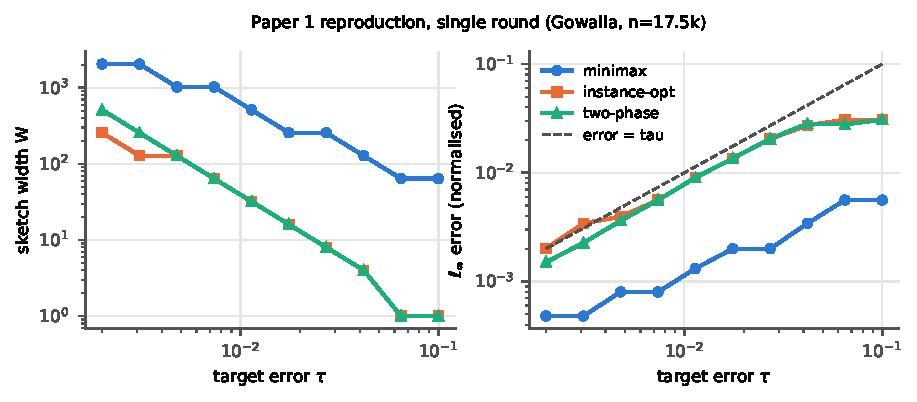
\includegraphics[width=0.56\textwidth]{repro_single.pdf}\hfill
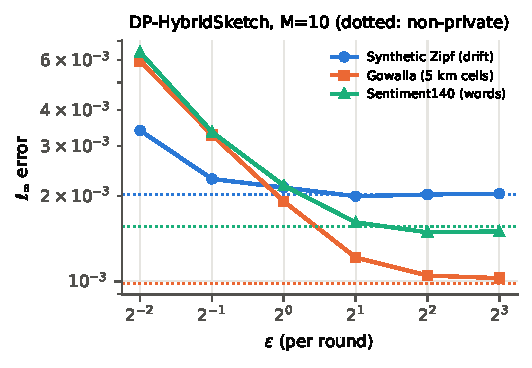
\includegraphics[width=0.36\textwidth]{repro_dp.pdf}\\[1mm]
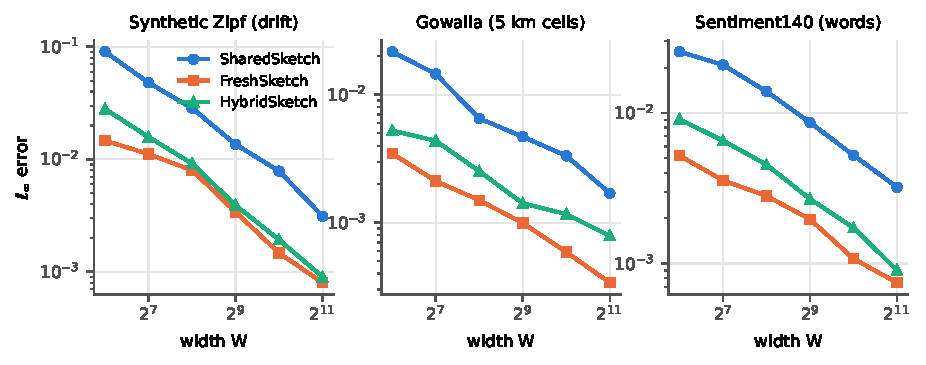
\includegraphics[width=0.75\textwidth]{repro_multi.pdf}
\caption{Reproduction of Wu et al. Top left: single-round width and error of the three width rules vs.\ target $\tau$ (Gowalla).
Top right: DP-HybridSketch error vs.\ $\eps$ (dotted: non-private). Bottom: multi-round $\ell_\infty$ vs.\ width for Shared, Fresh and Hybrid sketches.}
\label{fig:repro}
\end{figure*}
\begin{figure*}[t]\centering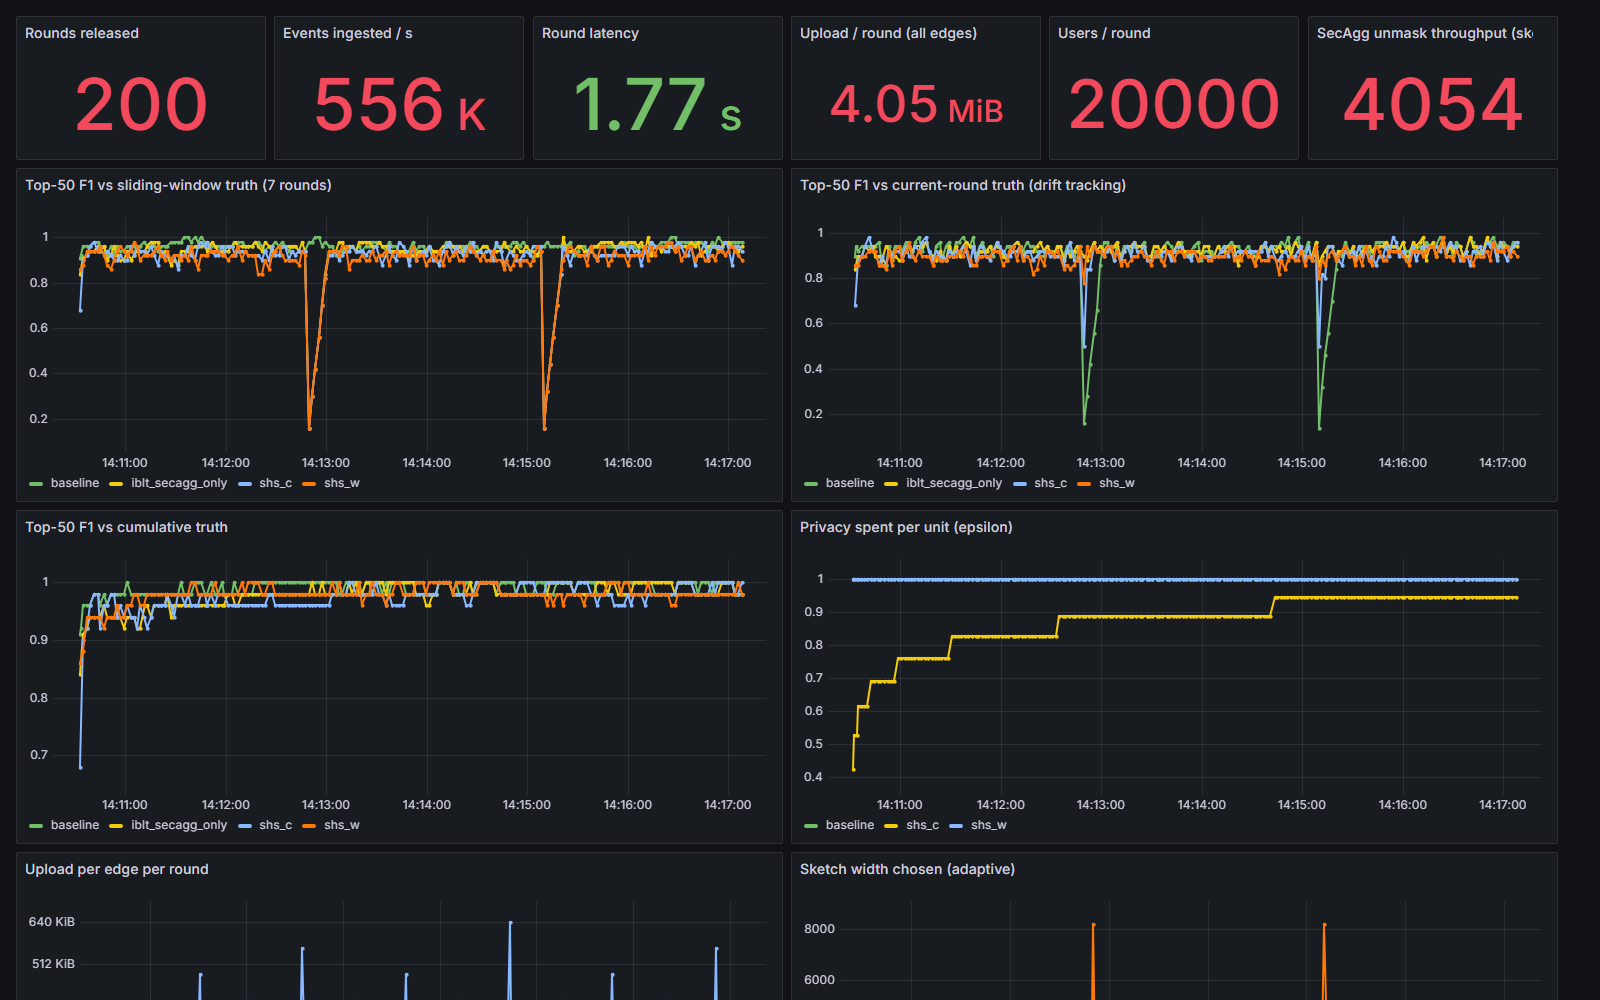
\includegraphics[width=0.66\textwidth]{grafana_dashboard.png}
\caption{Grafana dashboard of the 200-round live run (top part): headline counters, top-50 F1 per variant against sliding-window,
current-round and cumulative truth, and privacy spent. At both drifts the baseline (green) collapses on the current-round panel while
SHS-W/SHS-C recover within a round; SHS-W's window restart shows as a dip on the sliding-window panel.}\label{fig:grafana}
\end{figure*}
\section{Implementation}
\textbf{Data.} \emph{Gowalla} (SNAP) check-ins from 2010-01-01 to 2010-10-22, mapped to 0.05$^\circ$ grid cells as in~\cite{wu2023}:
6.1M events, 295 daily windows, $\sim$8.5k users/window, 80k items. \emph{Sentiment140}: 1.6M tweets as 22M word events (letters
only, truncated to 8 characters), 124 non-empty 6-hour windows, $\sim$9.8k users/window. \emph{Synthetic}: Zipf(1.1) over
100k items, 20k users/round, 200 rounds; the identities of the top-200 ranks are swapped with cold items at rounds 70
and 140. The Stack Overflow data of~\cite{gascon2023} (several GB via TFF) is replaced by the synthetic stream.

\textbf{Tools.} Kafka 3.7.0 (KRaft), Flower~\cite{beutel2020} 1.11.1, Python 3.11/NumPy 1.26, \texttt{cryptography} 42 (X25519, HKDF),
dp-accounting 0.4.4, confluent-kafka 2.4, InfluxDB 1.8, Grafana 10.4, all in a Docker Compose project.
\textbf{Configuration.} Depth $d{=}5$, baseline width 2048, 8 edges, top-$k{=}50$, sliding window 7 rounds, $\delta=10^{-6}$,
dictionary = items seen $\ge3$ times (the public candidate set assumed by~\cite{wu2023}). Unit tests verify mask
cancellation, IBLT linearity, exact folding and that noise-free tree sums equal a direct sketch of the union.

\section{Experimental Setup and Results}\label{sec:res}
\subsection{Reproduction of the base papers}
\begin{table}[t]\centering\footnotesize
\caption{Reproduction of Wu et al.~\cite{wu2023}. Single round: median width and fraction of trials with $\ell_\infty\le\tau$ over 10 targets $\tau$. Multi-round ($M{=}10$, $W{=}512$): normalised $\ell_\infty$ ($\times10^{-3}$).}\label{tab:repro}
\setlength{\tabcolsep}{3pt}\begin{tabular}{lrrrrrr}\toprule
 & \multicolumn{3}{c}{Median width (ok)} & \multicolumn{3}{c}{Multi-round $\ell_\infty$}\\\cmidrule(lr){2-4}\cmidrule(lr){5-7}
Dataset & minimax & inst.-opt & 2-phase & Shared & Fresh & Hybrid\\\midrule
Synthetic & 384 (1.00) & 48 (0.45) & 48 (0.76) & 13.58 & 3.40 & 3.90\\
Gowalla & 384 (1.00) & 24 (0.85) & 24 (0.96) & 4.69 & 0.99 & 1.41\\
Sentiment140 & 384 (1.00) & 48 (0.72) & 64 (0.92) & 8.65 & 1.97 & 2.68\\
\bottomrule\end{tabular}\end{table}
Table~\ref{tab:repro} and Fig.~\ref{fig:repro} reproduce Wu et al. In a single round, the two-phase rule picks widths 6--16$\times$
smaller than the minimax rule and close to the instance-optimal width, meeting the target error in 76--96\% of trials---the paper's
central single-round claim. In the multi-round setting HybridSketch beats SharedSketch by 3.2--3.5$\times$, as reported. Unlike the
paper, FreshSketch was 1.15--1.4$\times$ better than HybridSketch in our heterogeneous, time-ordered rounds at $d{=}5$; we report this
as a partial reproduction. DP-HybridSketch's error falls with $\eps$ and reaches the non-private error by $\eps\approx2$
(Fig.~\ref{fig:repro}, right). TrieHH (Table~\ref{tab:triehh}) discovers 39--223 words with precision 0.86--1.00 and recall@50 of
1.00 for $\eps\ge2$, matching the paper's trend; with a public dictionary, a one-shot DP CountSketch reaches recall@200 = 0.93 at
every $\eps$, which shows how much TrieHH pays for not needing a dictionary.
\begin{table}[t]\centering\footnotesize
\caption{TrieHH~\cite{zhu2020} on Sentiment140 ($n{=}659{,}775$ users, $\delta{=}1/n^2$): words discovered, recall of the true top-$k$ and precision of the discovered set w.r.t.\ the true top-200; DP-CountSketch with a public dictionary at the same $(\varepsilon,\delta)$ for reference.}\label{tab:triehh}
\setlength{\tabcolsep}{3pt}\begin{tabular}{rrrrrrr}\toprule
$\varepsilon$ & $\theta$ & found & R@50 & R@200 & P@200 & CS R@200\\\midrule
1 & 15 & 39 & 0.76 & 0.19 & 1.00 & 0.93\\
2 & 15 & 80 & 1.00 & 0.40 & 1.00 & 0.93\\
4 & 15 & 142 & 1.00 & 0.70 & 0.99 & 0.93\\
8 & 15 & 223 & 1.00 & 0.96 & 0.86 & 0.93\\
\bottomrule\end{tabular}\end{table}
\begin{table}[t]\centering\footnotesize
\caption{Recovery after the two abrupt drifts of the synthetic stream (mean of both; F1 vs.\ current-round top-50, $\varepsilon=1$).}\label{tab:drift}
\begin{tabular}{lrrrr}\toprule Variant & pre & min & rec.\ (rounds) & next 7\\\midrule
Baseline & 0.93 & 0.15 & 5.5 & 0.56\\
SHS-W & 0.90 & 0.60 & 1.5 & 0.85\\
SHS-C & 0.91 & 0.55 & 1.5 & 0.84\\
All components & 0.47 & 0.15 & 1.0 & 0.78\\
All $-$ drift det. & 0.49 & 0.08 & 7.5 & 0.24\\
\bottomrule\end{tabular}\end{table}
\begin{table}[t]\centering\footnotesize
\caption{System cost of the live run (synthetic stream, 2\,s per window, 8 edge containers and all services on one 12-core host).}\label{tab:system}
\begin{tabular}{lr}\toprule Metric & Value\\\midrule
Rounds (windows) processed & 200\\
Users / events per round & 20,000 / 20,000\\
Variants per round & 4\\
Round latency, median / p95 & 2.14 s / 2.28 s\\
Slowest edge: payload build (median) & 0.01 s\\
Slowest edge: wait for watermark (median) & 1.56 s\\
Server SecAgg unmask (median) & 1.6 ms\\
Upload per round, all 8 edges & 2.86 MiB\\
Kafka produce rate (median) & 499k events/s\\
\bottomrule\end{tabular}\end{table}
\begin{figure*}[t]\centering
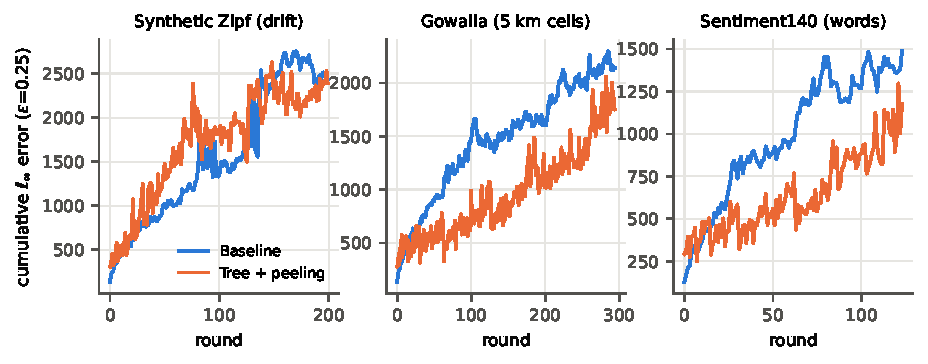
\includegraphics[width=0.49\textwidth]{cum_over_time.pdf}\hfill
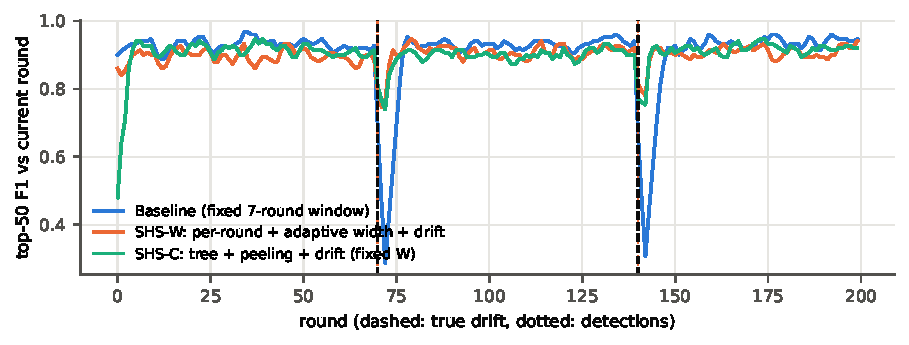
\includegraphics[width=0.49\textwidth]{drift.pdf}
\caption{Left: cumulative $\ell_\infty$ error over the stream at $\eps=0.25$, per-round release vs.\ tree release with peeling (\S\ref{sec:res}-B).
Right: top-50 F1 against the current round's truth on the synthetic stream ($\eps=1$, 3-round moving average); dashed lines mark the true drifts.}
\label{fig:cumtime}\label{fig:drift}
\end{figure*}
\begin{table*}[t]\centering\footnotesize
\caption{Streaming results at $\varepsilon=1$, $\delta=10^{-6}$ per unit over the whole stream (top-50, 7-round window, 8 edges). F1$_w$/F1$_n$: mean top-50 F1 against the sliding-window / current-round truth; F1$_c$: cumulative top-50 F1 over the second half; $\ell_\infty^c$: final cumulative $\ell_\infty$ error (counts); KiB: upload per edge per round.}\label{tab:main}
\setlength{\tabcolsep}{3.2pt}\begin{tabular}{lrrrrrrrrrrrrrrr}\toprule
 & \multicolumn{5}{c}{Synthetic} & \multicolumn{5}{c}{Gowalla} & \multicolumn{5}{c}{Sentiment140}\\
\cmidrule(lr){2-6} \cmidrule(lr){7-11} \cmidrule(lr){12-16}
Variant & F1$_w$ & F1$_n$ & F1$_c$ & $\ell_\infty^c$ & KiB & F1$_w$ & F1$_n$ & F1$_c$ & $\ell_\infty^c$ & KiB & F1$_w$ & F1$_n$ & F1$_c$ & $\ell_\infty^c$ & KiB\\\midrule
Baseline (DP-HybridSketch/round) & 0.96 & 0.91 & 0.99 & 1417 & 80 & 0.80 & 0.73 & 0.98 & 683 & 80 & 0.94 & 0.84 & 0.99 & 460 & 80\\
\textbf{SHS-W} (= all $-$ tree, $-$ peel) & 0.90 & 0.90 & 0.99 & 11066 & 31 & 0.79 & 0.72 & 0.96 & 745 & 55 & 0.81 & 0.75 & 0.98 & 686 & 54\\
\textbf{SHS-C} (= all $-$ adaptive width) & 0.90 & 0.90 & 0.99 & 2725 & 159 & 0.57 & 0.53 & 0.97 & 1604 & 159 & 0.73 & 0.69 & 0.98 & 1015 & 157\\
All components (tree+adapt+drift+peel) & 0.63 & 0.64 & 0.99 & 1215 & 83 & 0.45 & 0.43 & 0.98 & 977 & 115 & 0.67 & 0.64 & 0.99 & 534 & 172\\
\quad all $-$ drift detector & 0.41 & 0.40 & 0.97 & 3749 & 48 & 0.42 & 0.40 & 0.94 & 2090 & 75 & 0.86 & 0.78 & 0.98 & 1122 & 74\\
\quad all $-$ peeling & 0.75 & 0.76 & 0.98 & 2586 & 87 & 0.54 & 0.51 & 0.98 & 3440 & 99 & 0.71 & 0.67 & 0.99 & 861 & 191\\
\midrule
Non-private reference & 0.99 & 0.92 & 1.00 & 2026 & 80 & 0.98 & 0.81 & 1.00 & 266 & 80 & 0.99 & 0.85 & 1.00 & 360 & 80\\
\bottomrule\end{tabular}\end{table*}
\begin{figure*}[t]\centering
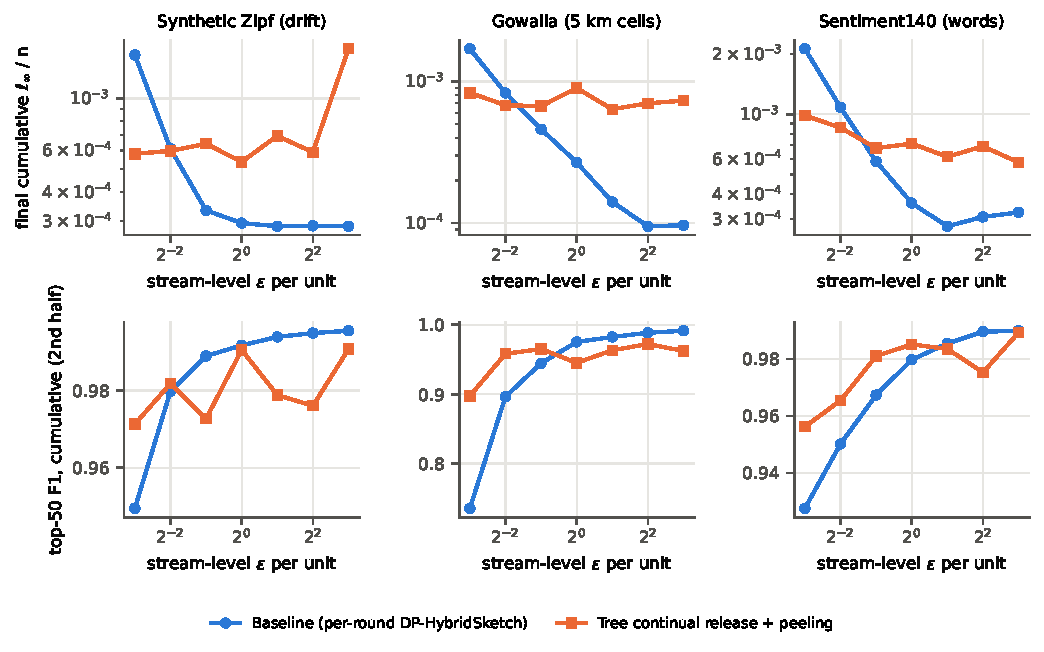
\includegraphics[width=0.58\textwidth]{eps_sweep.pdf}
\caption{Final cumulative $\ell_\infty$ (normalised, top) and second-half cumulative top-50 F1 (bottom) vs.\ stream-level $\eps$.}
\label{fig:eps}
\end{figure*}

\subsection{Streaming: baseline vs.\ enhancements}
\begin{figure*}[t]\centering
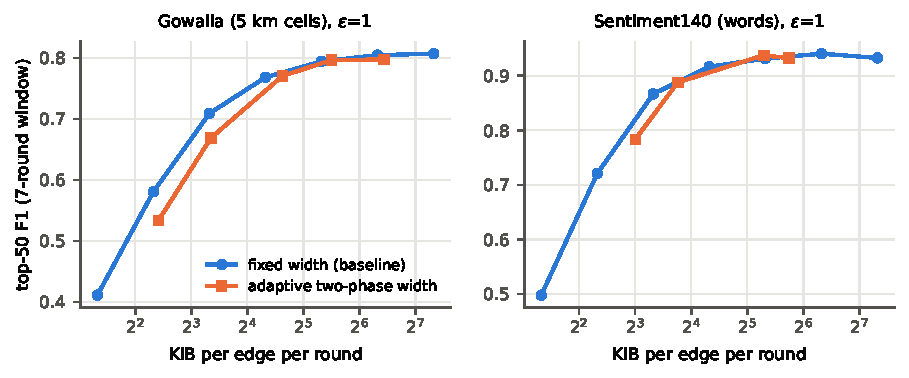
\includegraphics[width=0.40\textwidth]{comm_adaptive.pdf}\hfill
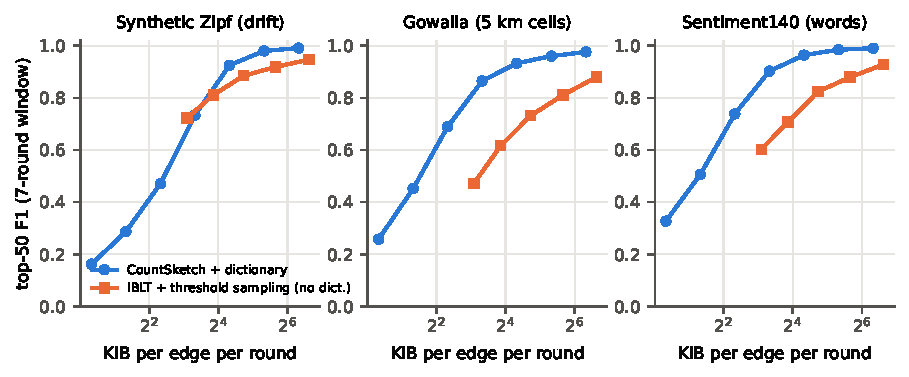
\includegraphics[width=0.58\textwidth]{hh_comm.pdf}
\caption{Left: window F1 vs.\ upload, fixed vs.\ adaptive width ($\eps=1$). Right: no-DP heavy hitters, CountSketch+dictionary vs.\ IBLT.}
\label{fig:comm}
\end{figure*}
Table~\ref{tab:main} reports all variants at $\eps=1$. \textbf{SHS-W} keeps the baseline's window F1 on Gowalla (0.79 vs.\ 0.80)
with 31\% less upload (55 vs.\ 80\,KiB per edge per round) and uses 2.6$\times$ less on the synthetic stream at a 0.06 F1 cost.
On Sentiment140 it loses 0.13 window F1 because the drift detector fires on organic topic shifts and shortens the window.
\textbf{SHS-C} matches the baseline on cumulative F1 but has lower window F1 at $\eps{=}1$. Combining every component is worse than
either recommended configuration: adaptive width picks narrow sketches from noisy releases, and shared-sign tree nodes cannot
tolerate them. Removing peeling from the full combination raises its cumulative error 1.6--3.5$\times$.

\textbf{Privacy--accuracy over time.} Table~\ref{tab:eps} and Fig.~\ref{fig:eps} vary the stream-level budget. With per-round
release, noise accumulates over the $t$ windows of a cumulative query; with the tree it grows with $\log t$. At
$\eps{=}0.125$ the tree with peeling cuts the final cumulative $\ell_\infty$ error by 2.0--2.6$\times$ and raises second-half
cumulative F1 on Gowalla from 0.74 to 0.90; at $\eps{=}0.25$ the gain shrinks to 1.0--1.3$\times$, and from $\eps\ge0.5$ the baseline is better: noise is no longer dominant,
and the tree's shared-sign collision floor ($\approx6\times10^{-4}n$) remains. For short sliding windows the per-round release
always wins, since a 7-round window needs only 7 noisy sketches while the tree needs up to 4 nodes at $\sqrt{h{+}1}\times$ more noise each.
Fig.~\ref{fig:cumtime} shows the mechanism behind the cumulative result at $\eps{=}0.25$: the baseline's cumulative error keeps growing with
the number of summed noisy rounds, while the tree's error stays flat after the first few levels are filled.
\begin{table}[t]\centering\footnotesize
\caption{Final cumulative $\ell_\infty$ error (counts) vs.\ stream-level $\varepsilon$: per-round release (B) vs.\ tree + peeling (T). Bold: lower.}\label{tab:eps}
\setlength{\tabcolsep}{3pt}\begin{tabular}{rrrrrrr}\toprule
 & \multicolumn{2}{c}{Synthetic} & \multicolumn{2}{c}{Gowalla} & \multicolumn{2}{c}{Sentiment140}\\
$\varepsilon$ & B & T & B & T & B & T\\\midrule
0.125 & 6119 & \textbf{2324} & 4394 & \textbf{2146} & 2913 & \textbf{1354}\\
0.25 & 2443 & \textbf{2392} & 2139 & \textbf{1755} & 1486 & \textbf{1177}\\
0.5 & \textbf{1335} & 2565 & \textbf{1188} & 1728 & \textbf{801} & 931\\
1 & \textbf{1179} & 2149 & \textbf{693} & 2319 & \textbf{495} & 981\\
2 & \textbf{1144} & 2770 & \textbf{364} & 1643 & \textbf{380} & 843\\
4 & \textbf{1148} & 2361 & \textbf{245} & 1810 & \textbf{423} & 951\\
8 & \textbf{1143} & 6507 & \textbf{249} & 1890 & \textbf{445} & 790\\
\bottomrule\end{tabular}\end{table}

\textbf{Drift.} Fig.~\ref{fig:drift} and Table~\ref{tab:drift}: on the synthetic stream the detector fires exactly at rounds 70 and 140
with no false alarms. The baseline's fixed window drops to F1 0.15 and needs 5.5 rounds to recover; SHS-W and SHS-C bottom out at
0.55--0.60 and recover in 1.5 rounds, raising mean F1 over the seven post-drift rounds from 0.56 to 0.84--0.85.

\textbf{Communication.} Fig.~\ref{fig:comm} (left) sweeps fixed widths against adaptive targets at $\eps=1$: adaptive width lies on
or just below the fixed-width frontier, so its value is choosing a good operating point without per-dataset tuning, not beating the
best width chosen in hindsight. Fig.~\ref{fig:comm} (right) evaluates heavy-hitter recovery without DP. On real data the IBLT needs
2--4$\times$ more upload than a CountSketch for the same F1, and the gap closes on the synthetic stream. Its benefit is that it
needs no dictionary (Paper~3 compared against a CountSketch without one).

\subsection{Live pipeline and system cost}
Table~\ref{tab:system} and Fig.~\ref{fig:grafana} come from a full live run on the synthetic stream with four variants side by side
(baseline, SHS-W, SHS-C and the SecAgg-only IBLT). Because the producer paces the replay at 2\,s per window, the median round latency (2.14\,s from dispatch to release, p95 2.28\,s) is mostly the edges waiting for the window's watermark (1.56\,s). Building a payload takes 12\,ms per edge and SecAgg unmasking 1.6\,ms at the server; the remaining $\approx$0.6\,s is Flower/gRPC transfer of 2.9\,MiB per round and server-side decoding of the four variants. The Kafka producer sustains $\approx$500k events/s, far above the stream rate, so the pipeline could replay much faster than real time. Replaying the same
configuration through the harness gives identical widths and payload sizes in every round and per-round F1 within 0.04 over all 200 rounds (top-$k$
ties), so the offline results describe the deployed pipeline.

\section{Discussion}
\textbf{What the results mean.} No single sketch configuration is best for all queries. Short-window and drift-sensitive statistics
favour per-round HybridSketch releases with drift-aware windows and adaptive width (SHS-W). Long-horizon cumulative statistics at
tight budgets favour tree release, but only with the peeling estimator, since tree sums lose HybridSketch's fresh-sign protection. The
communication savings of adaptive width are modest once a good fixed width is known; its value is not having to know it.

\textbf{Negative results.} (i) The tree loses at $\eps\ge1$ and on windows. (ii) Enabling all components at once is worse than SHS-W
or SHS-C. (iii) The IBLT layer is costlier than a dictionary-assisted CountSketch. (iv) FreshSketch beat HybridSketch in our multi-round reproduction.
(v) On Sentiment140 the drift detector raises false alarms that cost accuracy.

\textbf{Limitations and threats to validity.} SecAgg has no dropout recovery and noise seeds are deterministic for reproducibility. The
rounded distributed Gaussian is accounted as a continuous one. Guarantees are event-level, so user-level protection degrades with the number
of windows a user joins. The IBLT reveals sampled counts of decoded items. Gowalla is gridded and words are truncated, and the 8 edges are
cross-silo aggregators rather than individual devices. Results come from one seed per configuration (the reproduction experiments average 5--10 runs),
and the last-round $\ell_\infty$ is a single noisy sample.

\section{Conclusion and Future Work}
We built and evaluated a federated, privacy-preserving streaming heavy-hitter pipeline with real data flowing through Kafka, Flower,
secure aggregation and Grafana. We reproduced the core claims of the three base papers inside it and extended them for streams. The drift-aware
variant recovers from abrupt drift about 3.7$\times$ faster and saves up to 61\% upload. Tree release with peeling halves cumulative error at small
privacy budgets, and we mapped where each component stops helping. Future work: dropout-robust SecAgg (Flower SecAgg+), discrete Gaussian noise,
user-level accounting with participation caps, sign-hybrid trees, and DP candidate discovery that removes the public dictionary.

\begin{thebibliography}{00}
\bibitem{wu2023} J.~Wu, W.~Zhu, P.~Kairouz, and V.~Braverman, ``Private federated frequency estimation: Adapting to the hardness of the instance,'' in \emph{Proc. NeurIPS}, 2023.
\bibitem{zhu2020} W.~Zhu, P.~Kairouz, B.~McMahan, H.~Sun, and W.~Li, ``Federated heavy hitters discovery with differential privacy,'' in \emph{Proc. AISTATS}, PMLR 108, 2020.
\bibitem{gascon2023} A.~Gasc\'on, P.~Kairouz, Z.~Sun, and A.~T.~Suresh, ``Federated heavy hitter recovery under linear sketching,'' in \emph{ICML Workshop on Federated Learning}, 2023.
\bibitem{bonawitz2017} K.~Bonawitz \emph{et al.}, ``Practical secure aggregation for privacy-preserving machine learning,'' in \emph{Proc. ACM CCS}, 2017.
\bibitem{dwork2010} C.~Dwork, M.~Naor, T.~Pitassi, and G.~N.~Rothblum, ``Differential privacy under continual observation,'' in \emph{Proc. STOC}, 2010.
\bibitem{chan2011} T.-H.~H.~Chan, E.~Shi, and D.~Song, ``Private and continual release of statistics,'' \emph{ACM Trans. Inf. Syst. Secur.}, vol.~14, no.~3, 2011.
\bibitem{goodrich2011} M.~T.~Goodrich and M.~Mitzenmacher, ``Invertible Bloom lookup tables,'' in \emph{Proc. Allerton}, 2011.
\bibitem{charikar2002} M.~Charikar, K.~Chen, and M.~Farach-Colton, ``Finding frequent items in data streams,'' in \emph{Proc. ICALP}, 2002.
\bibitem{beutel2020} D.~J.~Beutel \emph{et al.}, ``Flower: A friendly federated learning research framework,'' arXiv:2007.14390, 2020.
\bibitem{mironov2017} I.~Mironov, ``R\'enyi differential privacy,'' in \emph{Proc. IEEE CSF}, 2017.
\end{thebibliography}

\end{document}
